\documentclass[12pt,a4paper]{article}
\usepackage[utf8]{inputenc}
\usepackage{amsmath}
\usepackage{geometry}
\usepackage{graphicx}
\usepackage{hyperref}
\usepackage{makeidx}

\usepackage{listings}
\usepackage{xcolor}
\usepackage{geometry}
\geometry{
	a4paper,
	total={170mm,257mm},
	left=25mm,
	top=25mm,
	right = 25mm,
	bottom = 25mm
}
\definecolor{codegreen}{rgb}{0,0.6,0}
\definecolor{codegray}{rgb}{0.5,0.5,0.5}
\definecolor{codepurple}{rgb}{0.58,0,0.82}
\definecolor{backcolour}{rgb}{0.95,0.95,0.92}

\lstdefinestyle{mystyle}{
	backgroundcolor=\color{backcolour},   
	commentstyle=\color{codegreen},
	keywordstyle=\color{magenta},
	numberstyle=\tiny\color{codegray},
	stringstyle=\color{codepurple},
	basicstyle=\ttfamily\footnotesize,
	breakatwhitespace=false,         
	breaklines=true,                 
	captionpos=b,                    
	keepspaces=true,                 
	numbers=left,                    
	numbersep=5pt,                  
	showspaces=false,                
	showstringspaces=false,
	showtabs=false,                  
	tabsize=2
}
\lstset{style=mystyle}
\makeindex
\begin{document}
	
	\begin{titlepage}
		\begin{center}
			\vspace*{1cm}
			
			\LARGE
			\textbf{Interactive Graphics}
			
			\large 
			\textbf{Final Course Project}
			
			\vspace{1.5cm}
			Authors: \\
			Sveva Pepe - 1743997 \\ 
			Simone Tedeschi - 1762897 \\
			Claudia Medaglia - 1758095 \\
			Christian Marinoni - 1745754
			\vfill
			
			
\includegraphics[width=0.7\textwidth]{logo}
			
			\vfill
			
			\large
			Professor: Marco Schaerf\break\break\break\break
			June 2020
			
		\end{center}
	\end{titlepage}
	
	\tableofcontents
	\pagebreak
	\section{Introduction}
	The goal of the project is to implement an interactive application 
	that makes use of basic WebGL or advanced libraries, as in our case ThreeJS. The project 
	cover the main aspects treated during the course, such as lights, textures, hierarchical models and animations.
	\section{Game}\label{g}
	We decided to develop a 3D version of ``Duck Hunt", a  
	famous game from the 80s, in which the objective is to hit  
	as many ducks as possible. We designed the
	scene as a first-person game, where the player is located 
	in a tall grass field and controls a rifle. 
	Thanks to the help of his dog, that frighten the ducks hidden 
	in the tall grass, the hunt can start. 
	The game ends when the player miss five ducks.
	In addition, our game provides other functionalities like enable 
	and disable sounds, pause the game or restart it.
	\\ \\The above described scene is depicted in the following figure:
	\begin{figure}[hbt!]
		\centering
		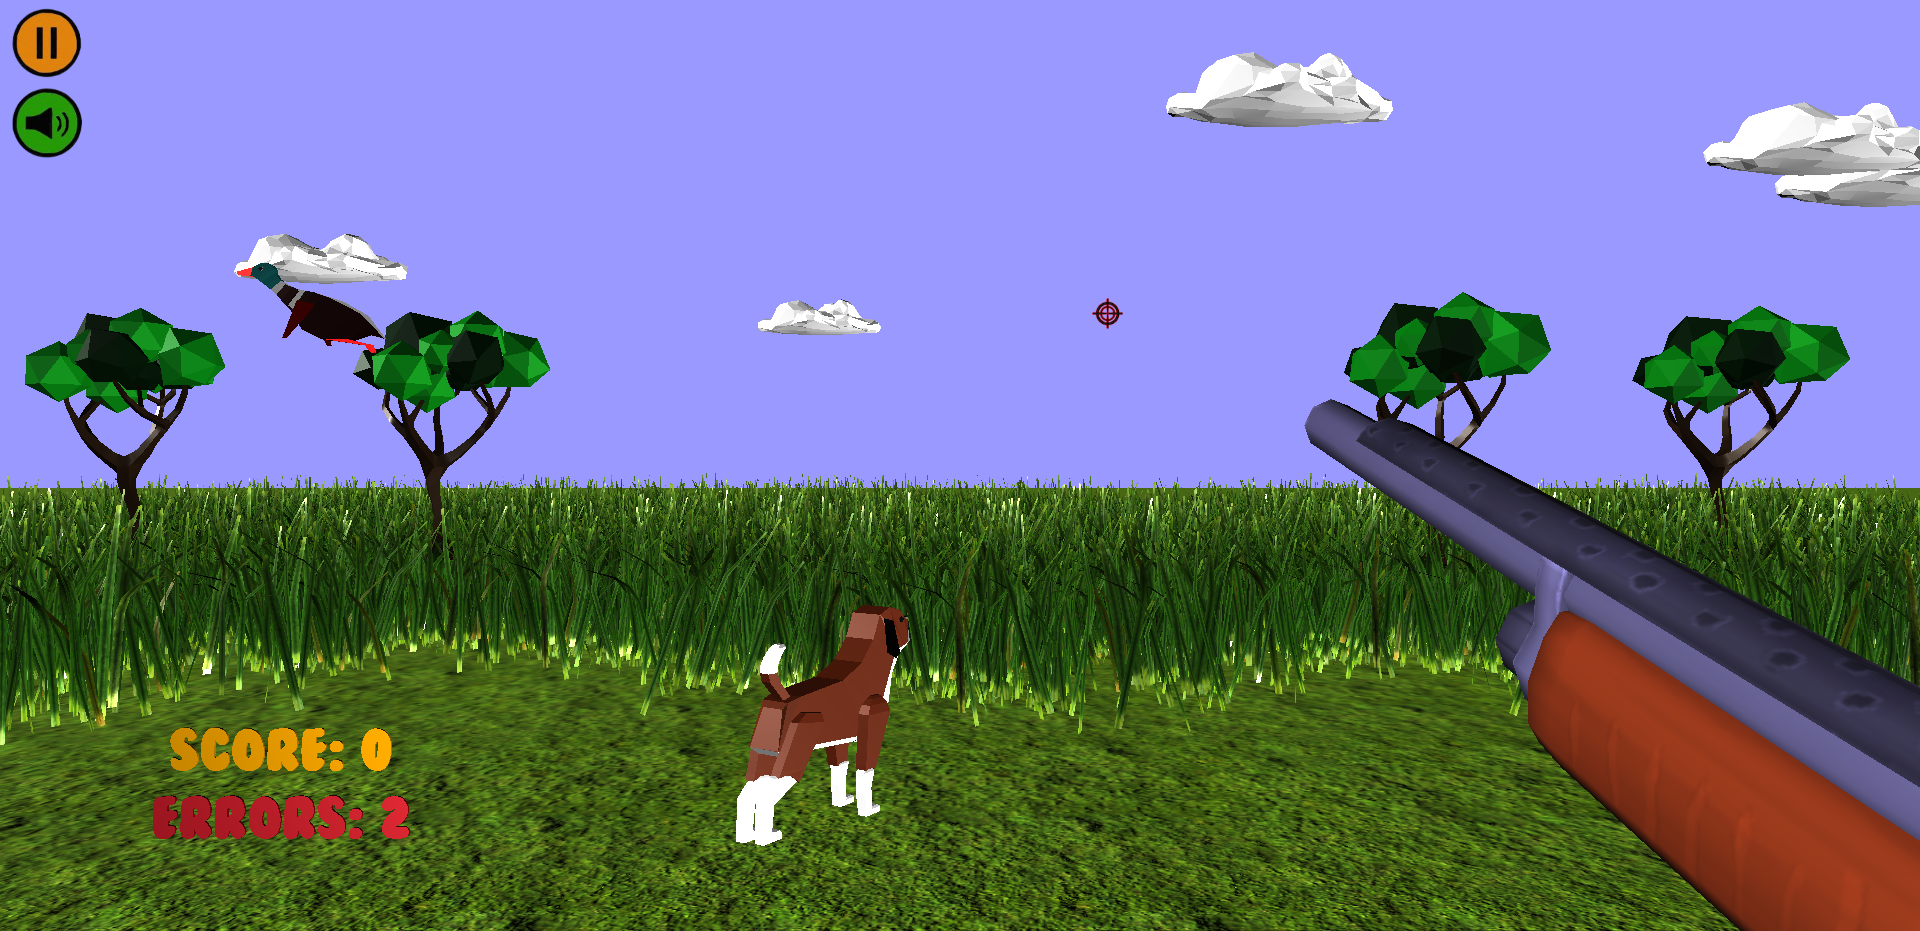
\includegraphics[width=1\textwidth]{game.png}
		\caption{Starting scene of the game.}
		\label{fig1}
	\end{figure}
	\section{Scene}
	The scene shown in Figure \ref{fig1}, which is a ThreeJS object, 
	has been obtained adding textures, lights, and different 3D models. 
	The dog and the ducks are hand-made models while the other are 
	taken from SketchFab. We used perspective camera to make the scene 
	as realistic as possible to let the center of projection coincide 
	with the user’s eyes.
	The prospective uses as parameters: \textit{fovy, aspect, near and 
		far}. \textit{Fovy}, which stands for ``field of view y-axis",
	identifies how wide the eyes open along the y direction.
	\textit{Aspect} represent the ratio between the width and height
	of the canvas.
	\textit{Near} and \textit{far} are any positive numbers 
	representing the minimum and maximum distances of the object, 
	with the restriction that near is always less than far.
	For the camera is defined also the  
	\textit{lookAt(x, y, z)} method, where the \textit{x, y} and \textit{z} 
	are the coordinates of the scene.
	The texts on the bottom right corner instead, have beed modeled using
	TTFLoader of ThreeJS, where through a Mesh the relative 
	colors have been applied.
	Moreover, in order to make our application responsive we add a 
	dedicated Listener to adapt the window size based on the device
	resolution. Finally, to improve the user experience antialiasing 
	has been used.
	\subsection{Lights and Textures}
	The ground texture was created by repeatedly applying a texture on 
	a plane, using a TextureLoader. Then, the texture is added to the
	scene through the use of meshes that map texture coordinates into
	world coordinates.\\
	A normal map has also been added to the \textit{MeshStandardMaterial} associated with the floor, useful for creating more realistic lighting effects, as well as a displacement map, which modifies - albeit slightly - the position of the vertices of the mesh.\\
	For the various models of the scene, the textures were imported with the model itself. For the sky, represented by a plane, a material was used which is associated with the desired blue colour.\\\\
	Three directional lights have also been added to the scene. 
	Two of them were placed on the left upper and bottom right corner 
	respectively of the scene to reproduce a sunny day, otherwise using
	only one of them we obtain either dark clouds or dark objects. 
	The third one has been introduced to illuminate texts because they 
	are ahead of other elements and so the previous lights were
	not able to light up also them.
	\section{3D Models}
	In this section we explain the models we have included in our project. They are splitted into
	the following two categories: 
	\begin{itemize}
		\item linear models: objects that are treated as an atomic entity;
		\item hierarchical models: objects composed by various sub-objects. 
	\end{itemize}
	\subsection{Linear Models} \label{linear}
	The linear models are models that are treated as singles entities. In our game are present the following four groups of linear models: Rifle, Trees, Clouds and Bushes. They contain 1, 4, 5 and 11 instances respectively that can be observed in Figure \ref{fig1}. We did this categorization to handle different kinds of objects in different ways, because objects belonging to different groups are indipendent to each other. Trees/bushes positions and orientations have been preset and remain static along the entire gameplay. Clouds positions instead, vary over time and rifle orientation can be controlled by the user. These last two aspects will be further explained in Sections \ref{anim} and \ref{user} where we will provide technical details.
	\subsection{Hierarchical Models}
	Hierarchical models are models composed by different sub-objects that allow to represent relationships between such objects. The major benefit of hierarchical structures is the possibility to handle animations in a simple and efficient way, because, for instance, if we want to apply a rotation to the whole object we need only to perform it to the root of the object itself, instead of applying n rotations to each individual component.
	\subsubsection{3D Duck Model}
	The first hierarchical model that we introduced in our project is an hand-made 3D model of a duck, created by us with Blender. Its structure is divided into four components: left and right wings, torso (including also the head) and legs. Such structure allowed us to reproduce the desired behavior, which consists in a simultaneous diagonal translation and a synchronous upward rotation of the wings. The above described hiearchical structure is shown in the following figure:
	\begin{figure}[hbt!]
		\centering
		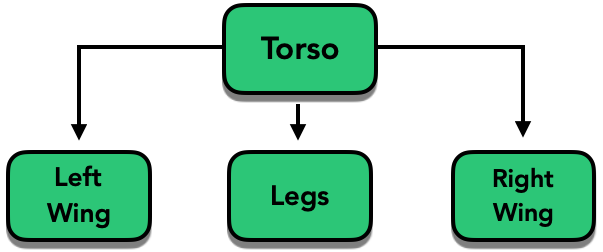
\includegraphics[width=0.7\textwidth]{hier_duck}
		\caption{Hierarchical model of the duck.}
		\label{fig2}
	\end{figure}
	
	\subsubsection{3D Dog Model}
	The second hierarchical model that we used in our project is again an hand-made 3D model created by us with Blender, representing a dog. Its structure is divided into ten components: left and right upper front legs, left and right upper back legs, left and right lower front legs, left and right lower back legs, torso (including also the head) and tail. 
	\\\\The hierarchical structure of the dog is depicted below: 
	\begin{figure}[hbt!]
		\centering
		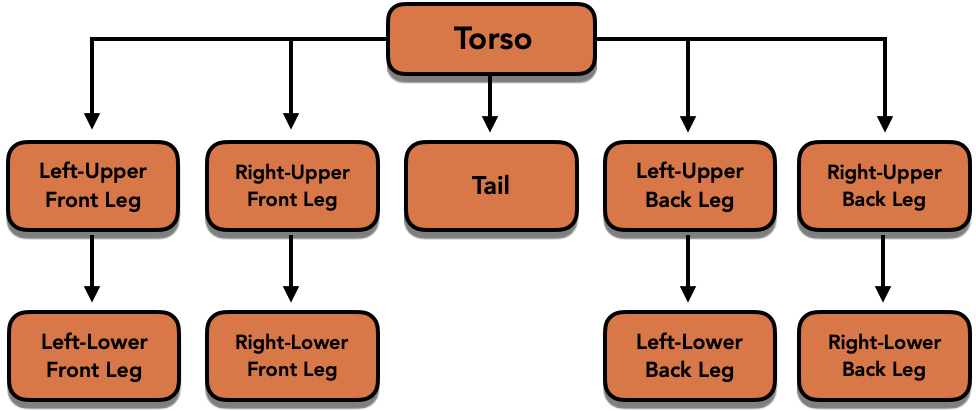
\includegraphics[width=0.98\textwidth]{hier_dog}
		\caption{Hierarchical model of the dog.}
		\label{fig3}
	\end{figure}
	\hfill \break We exploit such structure to let the dog move towards the bushes with few basic movements. To achieve this, we simply translate the ``Torso" node, which is the root of the hierarchy tree, and automatically all other components, which are attached to it, will follow its movement. In the meanwhile, we alternate the legs movements back and forth to reproduce a walk. Additional details will be provided in the Animations section (\ref{anim}).
	
	\section{Animations}\label{anim}
	Following the project requirements, we have integrated four different animations into the project:
	\begin{itemize}
		\item one for the ducks (both for the movement in the sky and for the wings);
		\item one for the dog;
		\item one for the clouds in the sky.
	\end{itemize}
	For each animation, we have developed different solutions to ensure an effective, scalable (and not impossible to obtain) result.	
	\subsection{Ducks animation}\label{da}
	The ducks animation is the most complex one, because it can be conceptually divided into two phases: the flight of the duck with the corresponding movement of the wings and its fall once hit.\\ 
	At each level, a specific number of ducks, among the 15 available, is concurrently shown in the scene and individually animated starting their flight by appearing from the grass; moreover, to ensure low predictability of the starting point and flight path and to increase the perceived difficulty, we made the whole process random.\\
	Every time a duck is killed or it leaves the scene, a new one is automatically generated to keep the sum of the currently shown ducks constant during the level.\\
	\\
	The translatory movement of the ducks in the sky was obtained by interpolating a keyframe sequence. 
	The starting position is a point having fixed y and z components and x component randomly extracted in the [-1.1) range; in this way, all ducks will start their flight from the same depth and height (more formally, they are positioned on the straight line given by the intersection of the planes $y=-0.2$ and $z=0$).\\
	A second point is then selected, which differs by the y component and which is used to generate the trajectory. Finally, a keyframe sequence is automatically generated and saved in the i-th element of the \textit{x\_keyFramesDucks} and \textit{y\_keyFramesDucks} arrays.\\
	These operations are carried out by calling, respectively, the \textit{chooseStartingPoint}, the \textit{chooseDirection} and the \textit{generateKeyFrames} functions within the \textit{animationBirds} function, which is responsible for updating the position of the ducks and the rotation of the wings.
	The path of each duck is interrupted as soon as its position is outside the camera's field of view; to verify this, a frustum and the containsPoint method were used.\\
	\\
	While translation is applied to the entire hierarchical model, wing rotation is applied to each wing individually. At first, we had implemented a solution based on keyframes, however, we saw that the final result was not good at all.\\
	So we preferred to use a gradual increase (decrease) within two defined values. Each wing is managed individually and its rotation values are reset as soon as the duck is ``removed" from the game.\\
	In this first part of the animation, we also made a distinction between left and right wing, and between a duck flying to the right and a duck going to the left.\\
	\\
	If the rifle strikes a duck then the second part of the animation takes place: the bird starts falling by translating downward and by rotating along the x-axis. In this case, since it is dead, the wings do not move to make everything more realistic.\\
	Finally, the duck is made no more visible when it reaches the ground.\\ 
	Once again, the animation does not involve keyframes but it is simply computed by decreasing the x component of the rotation and the y component of the position. 
	\subsection{Dog animation}
	Also for the dog, the animation consists of three types of movement:
	\begin{itemize}
		\item the translation of the entire dog group into the space;
		\item the rotation of the upper and lower part of the legs;
		\item the tail wagging.
	\end{itemize}
	Moreover, the animation consists of three phases:
	\begin{itemize}
		\item at the beginning of the first level, the dog enters the scene walking. Its presence is also functional since ideally its barking causes the ducks to start flying;
		\item the dog maintains his position throughout the game, wagging his tail in the meantime;
		\item after the game over, the dog moves and leaves the scene.
	\end{itemize}
	All these animations were achieved by setting keyframes manually. 
	
	\subsection{Clouds animation}
	The clouds animation is executed only during the gaming phase and it is interrupted when the game is paused or ends.\\
	Each cloud is moved individually, however, their animation can be divided into two modalities: those that have to go to the left will see the x component of their position decrease over time, the clouds that have to go to the right will see the x component increase.\\
	This x component is increased (decreased) until it is lower than (greater than) a certain threshold, after which the position of the cloud is restored to a predefined value, from which the process is repeated again.\\
	The threshold is set according to the position of the cloud: those with a lower z (i.e. placed further away from the camera) need to travel a greater distance before ``exiting" the screen.
	
	
	\section{User Interaction} \label{user}
	\subsection{Rifle}
	The 3D model of the rifle is positioned on the right of the camera and it is only partially visible with the aim to simulate a FPS (first-person shooter) game.
	When moving the mouse an event is launched and the mouseMove function is called.\\
	This function
	\begin{itemize}
		\item computes the mouse position on the screen;
		\item generates a ray passing to the mouse position by using the Threejs Raycaster object;
		\item this ray intersects a previously defined plane (which is the same where the duck trajectories are generated on);
		\item passes the intersection point to the LookAt function in order to rotate the rifle to face that point in world space.
	\end{itemize}
	Moreover, to make the game experience more realistic, a gunsight is used as a cursor. 
	When the user clicks the mouse a ``shoot" is generated. If the intersection point matches with a point of a duck mesh, that duck is killed and the ``falling" animation described above (\ref{da}) is executed. In any case, a ``bullet" (a white sphere) appears for some milliseconds on the screen.
	
	\subsection{Levels}
	As explained in Section \ref{g}, the game goal is to hit as many ducks as possible and every time a duck dies, the score is increased by one. When the user achieves a specific amount of points, a new level is reached and a ``Level X" text, generated through TextGeometry, is shown in the scene.\\
	Ideally, the game can be played for an infinite number of levels, with an increasing difficulty which depends on the number of simultaneously shown ducks, their speed and the quantity of points to reach.\\
	Each time a duck exits the screen without being shot, one of the five available errors is lost.\\ When the player misses five ducks, the game ends and the ``Game Over" text is shown.
	
	\subsection{Start \& Game Over menus}
	When the application starts, a white ``Start" box immediately appears.\\
	We put our logo on the center of the box; then the user can click on ``Start Game" to begin to play: basically when this is done, the box is no more visible and the game can really start. \\
	Otherwise he can learn ``How to play" or go to ``Credits" in order to know something more about us.\\
	Instead when the player finishes his chances, after the ``Game Over" text, it appears a ``Game Over" box through which he can read his current and his best scores and finally have the opportunity to play again.
	
	\subsection{Pause}
	While playing, the user can pause the game in whatever moment, except during the ``level up" and ``game over" phases.\\
	It is possible by clicking the button positioned on the top left corner of the screen to which a listener event is associated.\\
	When pausing the game, a TextGeometry representing the word ``pause" is created and shown at the centre of the screen.\\
	When the game is paused, it is not possible to kill the ``frozen" ducks, which will then return to action as soon as the pause is finished.\\
	Finally, the pause can also be activated by clicking the P key on the keyboard. The operation mode of the keyboard commands is the same as that of the button.
	\subsection{Sounds}
	We have also decided to add music and sounds to our game that the user can turn on and off at any time with the aim of making the player experience as interactive as possible.\\
	This is basically done by creating five HTML audio objects and by switching between the play() and pause() methods.\\
	In particular when the application is loaded, the music is turned off and this can be seen from the symbol of the music button.\\
	If the player turns on the music the button music image changes and he can hear a lot of effects and audios:
	\begin{itemize}
		\item when the start box is present an introductory audio track is repeated in a loop (using the loop() method);
		\item while moving from one level to another there is another audio that ends with the dog barking;
		\item every time that the user clicks on the screen, it generates the sound of a shoot;
		\item if the user clicks the pause button there is a sound to warn that the game has been stopped or resumed;
		\item finally, when the player loses, during the ``Game Over" text, there is a sad audio that indicates that for the moment the game is ended. After this sound, the first audio starts again, until the ``Play Again" button is pressed.
	\end{itemize}
	
	
	\section{Conclusion}
	
	
\end{document}